\documentclass[oneside]{book}

\usepackage[spanish]{babel}
\usepackage[latin1]{inputenc}
\usepackage{amsthm}
\usepackage[pdftex]{graphicx}
\usepackage{epstopdf}
\usepackage{enumerate}
\usepackage{tikz}

\title{Re-evaluaci�n de acciones en sistemas multi-agente}

\author{Diego Marcovecchio (LU: 83815)\\Director: Dr. Alejandro J. Garc�a}

%\date{20 de Agosto de 2011}

\theoremstyle{definition}
\newtheorem{definicion}{Definici�n}[section]
\theoremstyle{example}
\newtheorem{ejemplo}{Ejemplo}[section]

\newcommand{\ie}{i.\,e.}
\newcommand{\etal}{\mbox{{\em et al.}}}
\newcommand{\eg}{e.\,g.}
\newcommand{\raya}{\rule{\textwidth}{.05mm}}
\newcommand{\eoe}{\begin{flushright}$\Box$\end{flushright}}
\newcommand{\marginnote}[1]{\marginpar{\frame{#1}}}
\newcommand{\new}{\marginpar{\frame{\sc new}}}


\newcommand{\DLP}{\mbox{DeLP}}
\newcommand{\DLPa}{\mbox{DeLP}}
\newcommand{\DLPas}{\mbox{DeLP(a)-strict}}
\newcommand{\DLPans}{\mbox{DeLP(a)-non-strict}}
\newcommand{\dlp}{\mbox{\it de.l.p.}}

\newcommand{\cree}{B}

\newcommand{\no}{\mbox{$\sim$}}
\newcommand{\negda}[1]{\mbox{\textsf{not}$#1$}}
\newcommand{\naf}{\p{$\backslash$+}}
\newcommand{\notj}{{not}}
\newcommand{\comp}[1]{\mbox{$\overline{#1}$}}
\newcommand{\simbcomp}{ $\stackrel{\comp{\ \ }}{\vrule width 0pt height.8ex}$ }

\newcommand{\p}[1]{{\small \tt #1}}

% DLP programs 
% strict rule
\newcommand{\srule}[2]{\mbox{$ #1\;\leftarrow\;#2$}}
%\newcommand{\fact}[1]{\mbox{$ #1$}}  % some cls files have \fact defined for other things 
\newcommand{\facto}[1]{\mbox{$ #1$}} % for compatibility when the reason above holds
% literal
\newcommand{\lit}[1]{\mbox{$ #1$}}
% defesible rule
\newcommand{\drule}[2]{\mbox{$ #1\; \defleftarrow \; #2$}}
\newcommand{\defleftarrow}{{\raise1.5pt\hbox{\tiny\defleft}}}
\newcommand{\defleft}{\mbox{---\hspace{-1.5pt}\raise.05pt\hbox{$<$}}}
% presumption
%\newcommand{\presum}[1]{\drule{#1}{true}}
\newcommand{\presum}[1]{\drule{#1}{}}
% inverted rules
\newcommand{\invleftarrow}{ $\hookleftarrow $ }
\newcommand{\irule}[2]{\mbox{$#1$ \invleftarrow $#2$}}
\newcommand{\dquery}[1]{\drule{}{#1}}

% Donald Nute rules
\newcommand{\rr}[2]{\mbox{$ #1 \Rightarrow #2 $}} % defeasible
\newcommand{\re}[2]{\mbox{$#1 \rightarrow #2 $}} % strict
\newcommand{\de}[2]{\mbox{$ #1 \leadsto #2$}} %defeater

% Programci�n en Logica Extendida
\newcommand{\ple}{\mbox{\sc PLE}}
\newcommand{\extclause}[2]{\mbox{ #1 $\leftarrow$ #2}}
\newcommand{\true}{$true$}

% flecha rebatible para la derecha
\newcommand{\defrightarrow}{\mbox{$\succ\!$---}}
\newcommand{\defarrow}{{\raise1.5pt\hbox{\tiny\defrightarrow}}}


% Argumentos
\newcommand{\ArgA}{\mbox{${\mathcal A}$}}
\newcommand{\Ap}{\mbox{\ArgA$'$}}
\newcommand{\ArgAo}{\mbox{${\mathcal A_0}$}}
\newcommand{\ArgAa}{\mbox{${\mathcal A_1}$}}
\newcommand{\ArgAb}{\mbox{${\mathcal A_2}$}}
\newcommand{\ArgAn}{\mbox{${\mathcal A_n}$}}
\newcommand{\ArgAi}{\mbox{${\mathcal A_i}$}}
\newcommand{\ArgAim}{\mbox{${\mathcal A_{i-1}}$}}
\newcommand{\ArgB}{\mbox{${\mathcal B}$}}
\newcommand{\ArgBo}{\mbox{${\mathcal B_0}$}}
\newcommand{\ArgBa}{\mbox{${\mathcal B_1}$}}
\newcommand{\ArgBb}{\mbox{${\mathcal B_2}$}}
\newcommand{\ArgBk}{\mbox{${\mathcal B_k}$}}
\newcommand{\ArgQ}{\mbox{${\mathcal Q}$}}
\newcommand{\ArgQo}{\mbox{${\mathcal Q_0}$}}
\newcommand{\ArgQa}{\mbox{${\mathcal Q_1}$}}
\newcommand{\ArgQb}{\mbox{${\mathcal Q_2}$}}
\newcommand{\ArgQk}{\mbox{${\mathcal Q_k}$}}
\newcommand{\ArgQn}{\mbox{${\mathcal Q_n}$}}
\newcommand{\ArgQi}{\mbox{${\mathcal Q_i}$}}
\newcommand{\ArgQim}{\mbox{${\mathcal Q_{i-1}}$}}
\newcommand{\AQ}{\mbox{$\langle \ArgA,\ArgQ \rangle $}}
\newcommand{\AoQo}{\mbox{$\langle \ArgAo,\ArgQo \rangle $}}
\newcommand{\AaQa}{\mbox{$\langle \ArgAa,\ArgQa \rangle $}}
\newcommand{\AbQb}{\mbox{$\langle \ArgAb,\ArgQb \rangle $}}
\newcommand{\AnQn}{\mbox{$\langle \ArgAn,\ArgQn \rangle $}}
\newcommand{\AiQi}{\mbox{$\langle \ArgAi,\ArgQi \rangle $}}
\newcommand{\AimQim}{\mbox{$\langle \ArgAim,\ArgQim \rangle $}}
\newcommand{\BaQa}{\mbox{$\langle \ArgBa,\ArgQa \rangle $}}
\newcommand{\BkQk}{\mbox{$\langle \ArgBk,\ArgQk \rangle $}}

\newcommand{\Argum}[2]{\mbox{$\langle #1, #2 \rangle $}}
\newcommand{\AS}[2]{$\langle \{#1\}, #2 \rangle $}
\newcommand{\bigAS}[2]{$\bigl\langle \{#1\}, #2 \bigr\rangle $}

\newcommand{\nlA}[1]{$$\mbox{#1}$$}

% Sets of rules
\newcommand{\Facts}{\mbox{$\Theta$}}       % Facts
\newcommand{\SRules}{\mbox{$\Omega$}}       % Stricts rules
\newcommand{\SSet}{\mbox{$\Pi$}}       % Stricts rules & facts
\newcommand{\SSg}{\mbox{${\SSet}_G$}}  % Stricts rules without facts 
\newcommand{\SSp}{\mbox{${\SSet}_P$}}  % set of facts
\newcommand{\DD}{\mbox{$\Delta$}}      % Defeasible rules
\newcommand{\SD}{\mbox{$(\SSet,\DD)$}} % sets of rules of a program 
\newcommand{\FSD}{\mbox{$(\Facts,\SRules,\DD)$}} % sets of rules of a program 
\newcommand{\Presumptions}{\mbox{$\Phi$}}   % 
\newcommand{\DDp}{\mbox{$\Delta^{+}$}}  % Defeasible rules and presumptions
\newcommand{\SDp}{\mbox{$(\SSet,\DDp)$}} % sets of rules of a program 
\newcommand{\FSDP}{\mbox{$(\Facts,\SRules,\DD,\Presumptions)$}} % sets of rules of a program 

\newcommand{\FySyD}{\mbox{\Facts\ $\cup$ \SSet\ $\cup$ \DD}}   
\newcommand{\SyD}{\mbox{\SSet\ $\cup$ \DD}}   
\newcommand{\SyA}{\mbox{\SSet\ $\cup$ \ArgA}}
\newcommand{\SyAp}{\mbox{\SSet\ $\cup$ \Ap}}
\newcommand{\SyArga}{\mbox{\SSet\ $\cup$ \Arga}}
\newcommand{\RR}{\mbox{$\mathcal R$}}
\newcommand{\PP}{\mbox{${\mathcal P}$}}
\newcommand{\PPa}{\mbox{${\mathcal P}_1$}}
\newcommand{\PPb}{\mbox{${\mathcal P}_2$}}
\newcommand{\PPc}{\mbox{${\mathcal P}_3$}}
\newcommand{\PPd}{\mbox{${\mathcal P}_4$}}
\newcommand{\FFi}{\mbox{${\mathcal F}_i$}}
\newcommand{\FF}{\mbox{${\mathcal F}$}}

\newcommand{\SyQaQ}{\mbox{$\SSet \cup \{\ArgQa\\,\ArgQ\}$}}


\begin{document}
%\lstset{frame=single}
\maketitle

%\null
%\vfill

%\setcounter{page}{0}
\tableofcontents

\chapter{Introducci�n}

\section{Enunciado}

El objetivo de este trabajo es presentar en detalle un esquema de resoluci�n de
conflictos a utilizar en el sistema desarrollado en el marco de MAPC 2011\footnote{Multi-Agent Programming
Contest 2011 - http://www.multiagentcontest.org/}, la representaci�n de la base
de conocimiento utilizada para ello, las decisiones de dise�o e implementaci�n
tomadas, sus fortalezas, debilidades, y posibilidades de trabajo a futuro para
mejorarlo. % mentira sobre multi-agentes y coordinacion, por que resulta copado, etc

El sistema de resoluci�n de conflictos funciona de manera local a cada agente,
y tiene como objetivo reconsiderar la acci�n a realizar por dicho agente, una
vez terminado el proceso de decisi�n, analizando las potenciales acciones del
resto de los compa�eros de equipo.

El trabajo estar� dividido en diferentes cap�tulos para una mejor organizaci�n. Comenzaremos dando un conjunto de definiciones de alto nivel y un marco te�rico (incluyendo un background formal y el contexto de desarrollo) sobre el que trabajaremos durante el resto de la tesis. A continuaci�n, presentaremos en detalle la arquitectura de los agentes utilizados en la competencia (incluyendo la entrada y salida de datos, las diferentes secciones de procesamiento, y la comunicacion con otros agentes), e introduciremos las modificaciones necesarias para agregar la resoluci�n de conflictos. Luego describiremos detalladamente dicho sistema, presentando la posibilidad y el marco teorico para su completa realizaci�on, sus ventajas respecto al resto de los mecanismos de coordinaci�n de la competencia, y algunas posibilidades de trabajo a futuro. Por �ltimo, discutiremos algunas conclusiones globales y alternativas de trabajo para la coordinaci�n en el sistema.


\chapter{Definiciones preeliminares} % Contexto de la tesis (background formal, y contexto del desarrollo
En este cap�tulo se revisar�n algunas definiciones de conceptos t�cnicos, para posteriormente utilizarlos sin ambiguedad durante el resto de la presentaci�n.

\section*{Agente inteligente}
Un agente es una entidad computacional aut�noma, que puede percibir su entorno a trav�s de sensores, y actuar en dicho entorno utilizando efectores. Usualmente, la informaci�n que un agente percibe de su entorno es s�lo parcial. Los agentes toman decisiones a partir de la informaci�n contenida en su base de conocimiento, siguiendo diferentes conjuntos de reglas propuestas, y act'uan de manera acorde a la decisi'on tomada. Dichas acciones, a su vez, pueden producir efectos en el entorno.\\
Actualmente los agentes tienen un campo de aplicaci�n muy amplio y existen
muchos tipos de agentes diferentes (por ejemplo: \textit{reactivos}, \textit{deliberativos},
\textit{inteligentes}, \textit{de interface}, \textit{colaborativos}), los cuales a su vez est�n
orientados a distintos entornos de aplicaci�n.\\
En la mayor�a de los casos, los agentes no existen por s� solos, sino que participan de un Sistema Multi-Agente (SMA).

%El objetivo particular de este proyecto es la aplicaci�n de Argumentaci�n para
%la implementaci�n de di�logos entre agentes inmersos en un escenario con
%objetivos determinados. Puntualmente, se enfocar� la investigaci�n a la
%plataforma propuesta en el Multi-Agent Programming Contest, un juego acad�mico
%donde agentes independientes compiten por diferentes objetivos.\\
%Sin embargo, el desarrollo de herramientas para implementar tales formalismos se encuentra en
%progreso y a un paso m�s lento. Adem�s, muchas de las herramientas disponibles
%carecen de una base formal y suelen ser simplemente un entorno de desarrollo
%amigable.\\
 En un SMA, varios agentes
interact�an para conseguir alg�n objetivo o realizar alguna tarea . En este
tipo de sistemas, cada agente tiene informaci�n incompleta y capacidades
limitadas, el control del sistema es distribuido, los datos est�n
descentralizados, y la computaci�n es asincr�nica. Adem�s, los agentes se
desenvuelven en un entorno din�mico y cambiante, el cual no puede predecirse y
se ve afectado por las acciones que son llevadas a cabo por los agentes y
tambi�n por humanos.\\
%Un aspecto importante en SMA es la comunicaci�n entre agentes, la cual puede
ser necesaria para que los agentes compitan o cooperen de acuerdo a sus metas
individuales.


\section*{Sistema Multi-Agente}
Es un sistema en el cual muchos agentes interact�an para conseguir alg�n objetivo o realizar alguna tarea com�n. En los
sistemas multiagente, cada agente tiene informaci�n incompleta y capacidades limitadas, el control del sistema es distribuido, los datos est�n descentralizados, y la computaci�n es asincr�nica. Los agentes se desenvuelven en un entorno din�mico y cambiante, el cual no puede predecirse y se ve afectado por las acciones que son llevadas a cabo. Los di�logos con otros agentes del mismo ambiente son, actualmente, un �rea de estudio intensivo.

\section*{Inteligencia Artificial Distribuida}
Es el estudio, construcci�n y aplicaci�n de Sistemas Multi-Agente.

\section*{Arquitectura BDI}
El modelo BDI (\textit{Belief-Desire-Intentions}) es tanto una teor�a como una arquitectura de agentes. Un agente BDI posee un conjunto de \textbf{creencias}, un conjunto de \textbf{deseos}, y otro de \textbf{intenciones}. Las intenciones representan un conjunto de alternativas que el agente posee para alcanzar sus metas, y tienen la propiedad de ser \textbf{persistentes}; el agente mantiene todas sus intenciones hasta que logre cumplirlas, o bien se de cuenta de que \textit{no} podr� cumplirlas, o bien, por alg�n otro motivo, las razones que tuvo para adoptar por primera vez a la intenci�n dejaron de ser v�lidas.\\
A grandes rasgos, la arquitectura BDI propone que el agente:
\begin{enumerate}
	\item Perciba los cambios del entorno en el que se desenvuelve.
	\item Revise sus creencias del mundo en base a la percepci�n.
	\item Razone acerca de sus intenciones para reconsiderarlas, de ser necesario.
	\item Seleccione una acci�n a seguir, razonando sobre sus creencias e intenciones.
	\item Ejecute la acci�n seleccionada, y vuelva al primer paso.
\end{enumerate}

\section*{Argumentaci�n rebatible}
La argumentaci�n rebatible es un mecanismo de razonamiento no mon�tono en donde
la aceptaci�n o el rechazo de una proposici�n dependen de un an�lisis entre
argumentos a favor y en contra de esa proposici�n. Usualmente es utilizada bajo
diferentes formalizaciones para capturar aspectos del razonamiento del sentido
com�n y la representaci�n de informaci�n incompleta y potencialmente
inconsistente.\\
En particular, la toma de decisiones de los agentes inteligentes realizada por nuestro equipo en el marco de la competencia MAPC 2011, fue realizada utilizando Argumentaci�n rebatible via DeLP. (cita!)

\section*{DeLP}
DeLP (Defeasible-Logic Programming) es...
%aca mentir MUCHO.

\section{Multi-Agent Programming Contest}
El \textit{Multi-Agent Programming Contest} es un concurso de programaci�n de
Inteligencia Artificial iniciado en el a�o 2005 con el objetivo de estimular la
investigaci�n en el �rea de desarrollo y programaci�n de Sistemas Multi-Agente.
Para ello, la competencia propone diferentes escenarios de juego de manera
anual, que obligan a los participantes tanto a identificar y resolver problemas
clave, como a explorar lenguajes, plataformas y herramientas de programaci�n
para Sistemas Multi-Agente.

\subsection{Escenario MAPC 2011}

El escenario del a�o 2011 est� formado por el mapa de un planeta representado
mediante un grafo. Cada nodo del grafo es una locaci�n v�lida (y tiene un valor
determinado), y existen arcos (con diferente costo de energ�a) que permiten a un
agente desplazarse de una locaci�n a otra.\\
En cada ronda de la competici�n participan dos equipos rivales. Cada equipo
posee un conjunto de agentes con diferentes roles preestablecidos
(\textit{Explorador}, \textit{Saboteador}, \textit{Reparador},
\textit{Sentinela} e \textit{Inspector}). El rol de cada agente define tanto el
conjunto de acciones que puede realizar, como sus caracter�sticas f�sicas
(\textit{Energ�a}, \textit{Salud}, \textit{Fuerza} y \textit{Rango de
Visi�n}).\\
\subsubsection{Puntaje}
La simulaci�n del juego se desarrolla por pasos, y en cada paso se otorga a los
equipos una determinada cantidad de puntos seg�n el estado de la simulaci�n. El
objetivo del juego es obtener la mayor cantidad de puntos posibles cuando la
simulaci�n termina.\\
Para obtener puntos, los agentes de cada uno de los equipos deben lograr formar
\textit{"`zonas"'} en el mapa logrando posicionarse en diferentes locaciones de
manera estrat�gica. La predominancia de un equipo sobre el otro en los nodos es
determinada por un algoritmo bien definido para la competencia, y el valor de
todos los nodos dominados por un equipo es el principal factor del puntaje
otorgado en cada uno de los pasos de la simulaci�n. Algunas otras situaciones,
como el logro de determinados \textit{achievements}, pueden otorgar puntos
adicionales y dinero al equipo.
\subsubsection{Acciones}
Todos los agentes tienen acciones en com�n que pueden realizar en cada uno de
los pasos de la simulaci�n:
\begin{itemize}
	\item goto(X): el agente se desplaza hacia el nodo X, siempre y cuando
exista un arco que conecte el nodo actual del agente con X, y dicho arco tenga
un costo menor a la energ�a actual del agente.
	\item survey(X): el agente recibe en su pr�xima percepci�n los costos de
todos los arcos conectados al nodo en el que se encuentra actualmente.
	\item buy(X): el agente utiliza el dinero obtenido a partir de los
\textit{achievements} para aumentar el valor m�ximo de cualquiera de sus
caracter�sticas f�sicas (Energ�a, Salud, Fuerza o Rango de visi�n) en 1 punto.
	\item recharge: el agente recupera el 20\% de su energ�a m'axima.
	\item skip: el agente pasa al turno siguiente sin realizar ning�n tipo
de acci�n.
\end{itemize}

Adem�s, seg�n el rol de cada agente, existen algunas acciones espec�ficas que
pueden realizar:
\begin{itemize}
	\item attack(X): acci�n disponible �nicamente para los \textit{Saboteadores}; el
agente ataca a un enemigo X, si dicho enemigo se encuentra en el mismo nodo. El
ataque, de tener �xito, decrementa la energ�a del agente enemigo, pudiendo
deshabilitarlo en caso de que �sta llegue a 0.
	\item parry: acci�n disponible �nicamente para los \textit{Reparadores},
\textit{Saboteadores} y \textit{Sentinelas}. La acci�n protege al agente de los ataques enemigos,
impidiendo que �stos tengan �xito.
	\item probe: acci�n disponible �nicamente para los \textit{Exploradores}. El
agente recibe en su pr�xima percepci�n el valor del nodo en el que se encuentra
actualmente. �sta acci�n no s�lo resulta importante por conocer el valor del
nodo, sino que adem�s permite que, cuando el nodo es conquistado por el equipo,
dicho valor se sume al total de puntos de la zona. Un nodo en el que no se
realiz� \textit{probe} suma �nicamente 1 punto al valor total de la zona.
	\item inspect: acci�n disponible �nicamente para los \texit{Inspectores}. El
inspector recibe en su pr�xima percepci�n la informaci�n f�sica (Salud, Energ�a,
Fuerza, Rango de visi�n) de todos los agentes enemigos que se encuentren en el
mismo nodo que �l, o en cualquier vecino directo.
	\item repair(X): acci�n disponible �nicamente para los \textit{Reparadores}. El
reparador aumenta el valor de la Salud actual de su compa�ero de equipo X
(volviendo a habilitarlo, en caso de que su Salud fuera 0).

\end{itemize}

\subsubsection{Toma de decisiones y motivaci�n para la resoluci�n de conflictos}
A diferencia de los a�os anteriores, esta competencia apunta a lograr un buen
Sistema Multi-Agente puramente distribuido; esto significa que cada agente debe
realizar el proceso de toma de decisiones por su cuenta, en lugar de
contar con una inteligencia centralizada que decida cu�l ser� la acci�n a
realizar para cada uno de los agentes.\\
Dado que cada agente decide por separado qu� acci�n tomar, muchas veces ocurre que dos (o m�s) de los agentes del mismo
equipo realizan acciones que resultan redundantes, peligrosas, y en el peor de
los casos, perjudiciales al combinarse. Si bien por limitaciones temporales 'unicamente se realizaron coordinaciones impl'icitas en las acciones de los agentes, es naturalmente posible mejorar dicha coordinaci'on para sacar mayor r'edito de las acciones.
\chapter{Arquitectura general del agente}

Este cap�tulo tiene el objetivo de analizar el dise�o y estructura que presenta el 
enfoque de agente propuesto. Primero desde un punto de vista general, para luego 
poner especial �nfasis en el m�dulo dedicado a la toma de decisiones, responsable 
del manejo de las creencias, deseos e intenciones. Ser�n presentados en detalle los 
componentes b�sicos del esquema BDI aplicado, as� como tambi�n las principales 
adaptaciones y agregados realizados en esta implementaci�n particular.

\section{Dise�o general}

%\label{sec:dise�oGeneral}

El programa agente presenta una estructura simple en cuanto a su divisi�n m�s general. 
Esto permite su entendimiento a nivel individual, al mismo tiempo que facilita su 
integraci�n en un entorno multi-agente como el enfrentado. La interacci�n con el entorno 
y el procesamiento inicial de la informaci�n recibida finalizan con la generaci�n de una 
serie de creencias que son incorporadas a la base de conocimiento mantenida por el agente. 
Este conjunto de creencias es empleado posteriormente por el m�dulo encargado de tomar 
decisiones. La forma en que se estructuran los componentes principales es detallada a 
continuaci�n.

\subsection{Estructura b�sica del agente}

%\label{sec:estructuraBasica}

El programa principal del agente es el encargado de manejar la comunicaci�n con los 
servidores, tanto el del juego como el de percepciones (presentado 
a continuaci�n). Tambi�n es responsable de parsear y procesar la informaci�n contenida 
en la percepci�n para darle el formato interpretado por la base de conocimientos, y 
enviar la acci�n que ha sido elegida por el m�dulo de toma de decisiones.

\begin{figure}
 \centering
 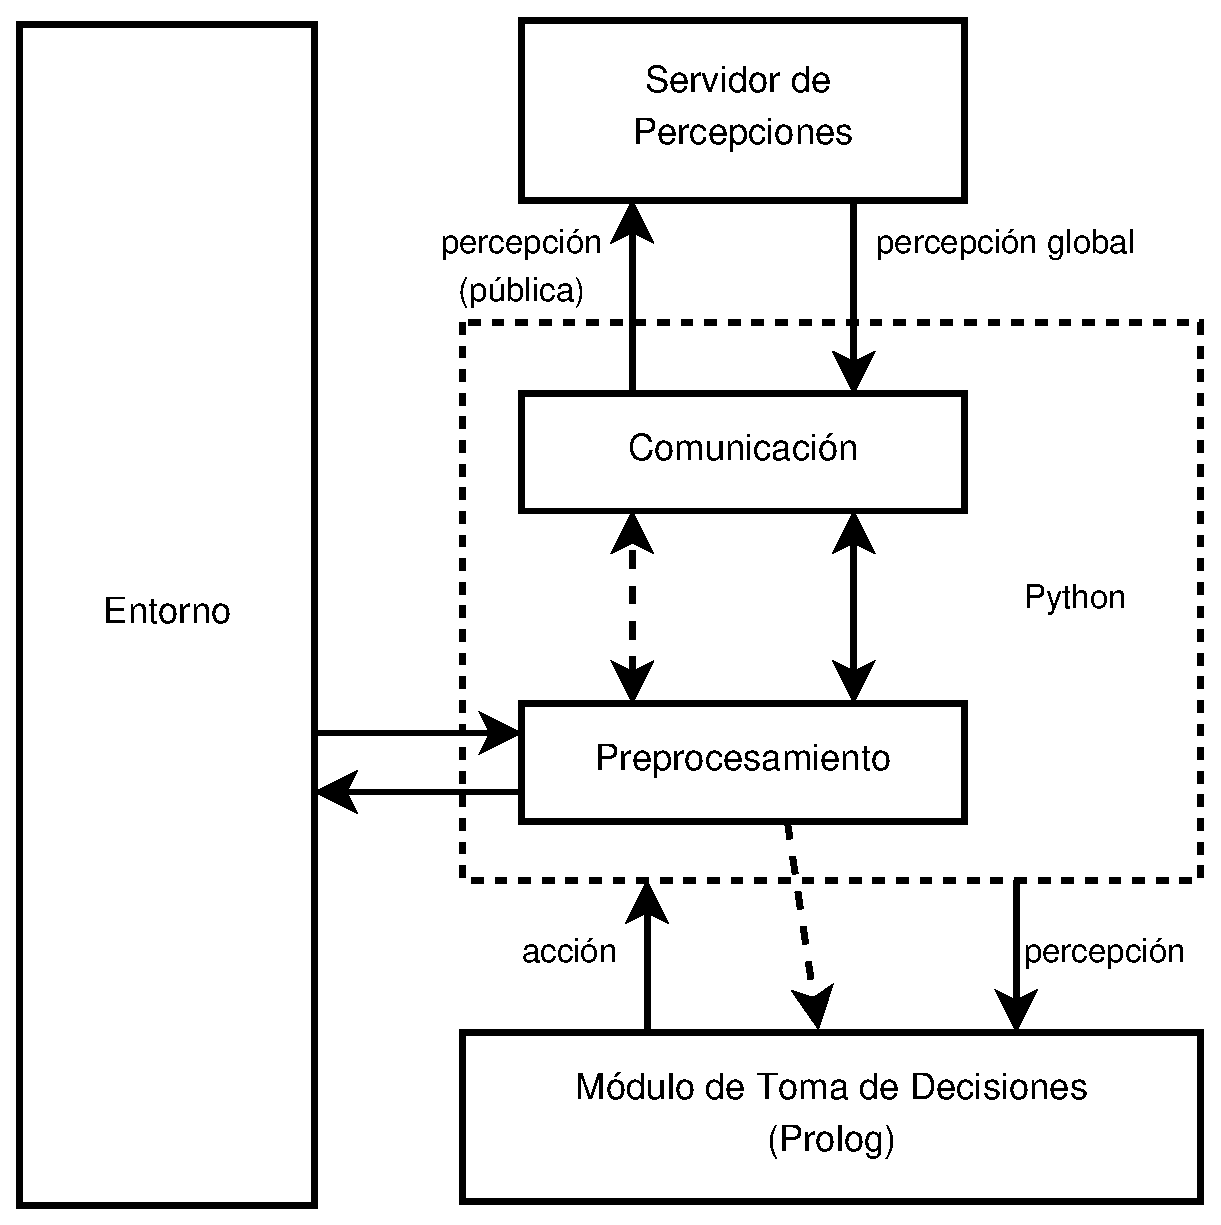
\includegraphics[scale=.4]{agent_architecture.eps}
 \caption{Diagrama de la arquitectura del agente. Las l�neas punteadas representan el 
 flujo de control, y las l�neas cont�nuas representan el flujo de datos.}
 \label{fig:architecture}
\end{figure}

El servidor de percepciones (SP) es un programa independiente, encargado de unificar las 
percepciones de todos los agentes que se encuentran en ejecuci�n. Recibe sus percepciones 
individuales y retorna a cada uno de ellos el conjunto de datos que a�n no poseen, de 
manera que todos los agentes del equipo cuenten con la misma informaci�n en cuanto al estado 
del escenario.

En cada iteraci�n de la simulaci�n, el agente recibe un mensaje por parte del servidor 
del juego, el cual contiene la informaci�n asociada a la percepci�n del turno en disputa. 
Este mensaje es parseado y traducido en una estructura que permite manipular los datos 
con mayor facilidad. Los datos son divididos en dos conjuntos, uno ``p�blico'', el cual 
es compartido con los dem�s agentes del equipo, y uno ``privado''. La secci�n p�blica de 
datos es compartida a trav�s del mencionado servidor de percepciones.

El agente une entonces su propia percepci�n con la percepci�n global recibida del servidor 
de percepciones, y genera un �nico conjunto de datos. Esta informaci�n es incorporada a la 
base de conocimientos, estableciendo nuevas creencias para el agente.

El m�dulo de toma de decisiones, analizado en la secci�n \ref{sec:arquitecturaBDI}, es el 
que implementa el modelo BDI respetado por el agente. Este m�dulo es consultado en cada 
iteraci�n para obtener la pr�xima acci�n a ser ejecutada. Una vez que el flujo de control 
retorna al programa principal, la acci�n seleccionada es enviada al servidor del juego.

\subsection{Base de conocimiento}

%\label{sec:baseConocimiento}

Como fue mencionado, la percepci�n del agente en cada iteraci�n es convertida a una 
estructura de datos que permite, de manera m�s sencilla, manipular y compartir la 
informaci�n. Cuando el agente cuenta con todos los datos relativos a las percepciones 
del equipo, la base de conocimiento puede ser actualizada convenientemente. Una colecci�n 
de predicados de Prolog consultados desde el programa principal se encarga de verificar 
que la informaci�n existente no resulte sobreescrita, y que informaci�n redundante no sea 
incorporada. 

La informaci�n que constituye conocimiento certero sobre el estado del escenario es 
almacenada mediante t�rminos, que sirven como par�metros %esto era ARGUMENTOS
del predicado \texttt{k/1} 
(\textit{knowledge}). Cada uno de los datos de inter�s es representado mediante un 
t�rmino diferente. 
En muchos casos, esta clase de t�rminos incluyen un par�metro%argumento
ligado al n�mero de turno
en el cual el dato fue percibido. De esta forma, es posible realizar ciertos an�lisis, 
como por ejemplo, considerar obsoleta la informaci�n de una determinada antig�edad.

	% En castellano para mantener el idioma y porque las b() 
	% est�n as�.
\begin{verbatim}    
    k(equipoAgente(Agente, Equipo)).
    k(valorNodo(Nodo, Valor)).
    k(arco(Nodo1, Nodo2, Costo)).
    k(posicionAgente(Agente, Turno, Posici�n)).
    k(equipoNodo(Turno, Nodo, Due�o)).    
\end{verbatim}

Las creencias que provienen de inferencias y c�lculos realizados a partir de informaci�n 
ya existente tambi�n son almacenadas mediante t�rminos, en este caso par�metros %argumentos
del predicado \texttt{b/1} (\textit{beliefs}). Este tipo de creencias es empleado directamente 
por el m�dulo encargado de la toma de decisiones, y se mantienen vigentes s�lo durante el 
turno en el cual fueron generadas. Es decir, que, al finalizar cada turno, son descartadas 
para evitar futuros problemas o inconcistencias.

\begin{verbatim}
    b(estoyEnLaFrontera).
    b(posibleExplorar(Nodo)).
    b(haySaboteador(Nodo)).
\end{verbatim}

Existe cierta informaci�n que es formulada de manera hipot�tica. Se trata de datos 
surgidos de suposiciones realizadas sobre posibles estados futuros del escenario, a partir 
de su estado actual. Este tipo de datos resulta fundamental para facilitar los c�lculos 
realizados por los algoritmos que se encargan de buscar formas de maximizar el puntaje 
del equipo. Dado que no constituye informaci�n real, sino posible a futuro, se almacena 
mediante par�metros %argumentos
de un predicado especial, \texttt{h/1} (\textit{hypothetical}).

\begin{verbatim}
    h(nodoEquipo(Nodo, Due�o)).
    h(posicion(Turno, Agente, Nodo)).    
\end{verbatim}

Las intenciones surgen del proceso argumentativo explicado m�s adelante, y son 
representadas utilizando t�rminos. Si la intenci�n no posee argumentos, entonces es 
representada mediante un �tomo. En otro caso, se emplea un functor que denota el 
nombre de la intenci�n, acompa�ado por un argumento. Las acciones, por el contrario, 
son representadas a trav�s de listas. El primer elemento de la lista es un at�mo denotando 
el tipo de acci�n. Y el resto de la lista contiene, ocacionalmente, un t�rmino que 
indica el argumento de la acci�n, como por ejemplo el nombre de un nodo o un agente.
Los planes son representados mediante listas de acciones, es decir, listas de listas.

Contrario a lo que ocurre con las creencias, tanto las intenciones como los planes 
constituyen informaci�n que debe perdurar en la base de conocimiento tantos turnos 
como sea necesario. Para este tipo de datos se emplean hechos espec�ficos que cuentan 
con un �nico argumento.

\begin{verbatim}
    intencion(explorar(vertex7)).
    plan([[recharge], [goto, vertex7], [survey]]).
\end{verbatim}

\section{Arquitectura BDI} %CAMBIAR: Toma de decisiones?

\label{sec:arquitecturaBDI}

El m�dulo de toma de decisiones es consultado por el programa principal, obtiene la 
pr�xima acci�n a ser ejecutada, y la retorna para que pueda ser enviada. Esta es una 
secuencia que se reitera en cada uno de los turnos de la simulaci�n, con una caracter�stica:
cuando es necesario plantear y planificar una nueva meta, intervienen una serie de 
componentes especiales, que difieren de aquellos involucrados cuando se cuenta con una 
meta ya planificada. Cada uno de estos componentes es descrito en esta secci�n.

\begin{figure}[h]
 \centering
 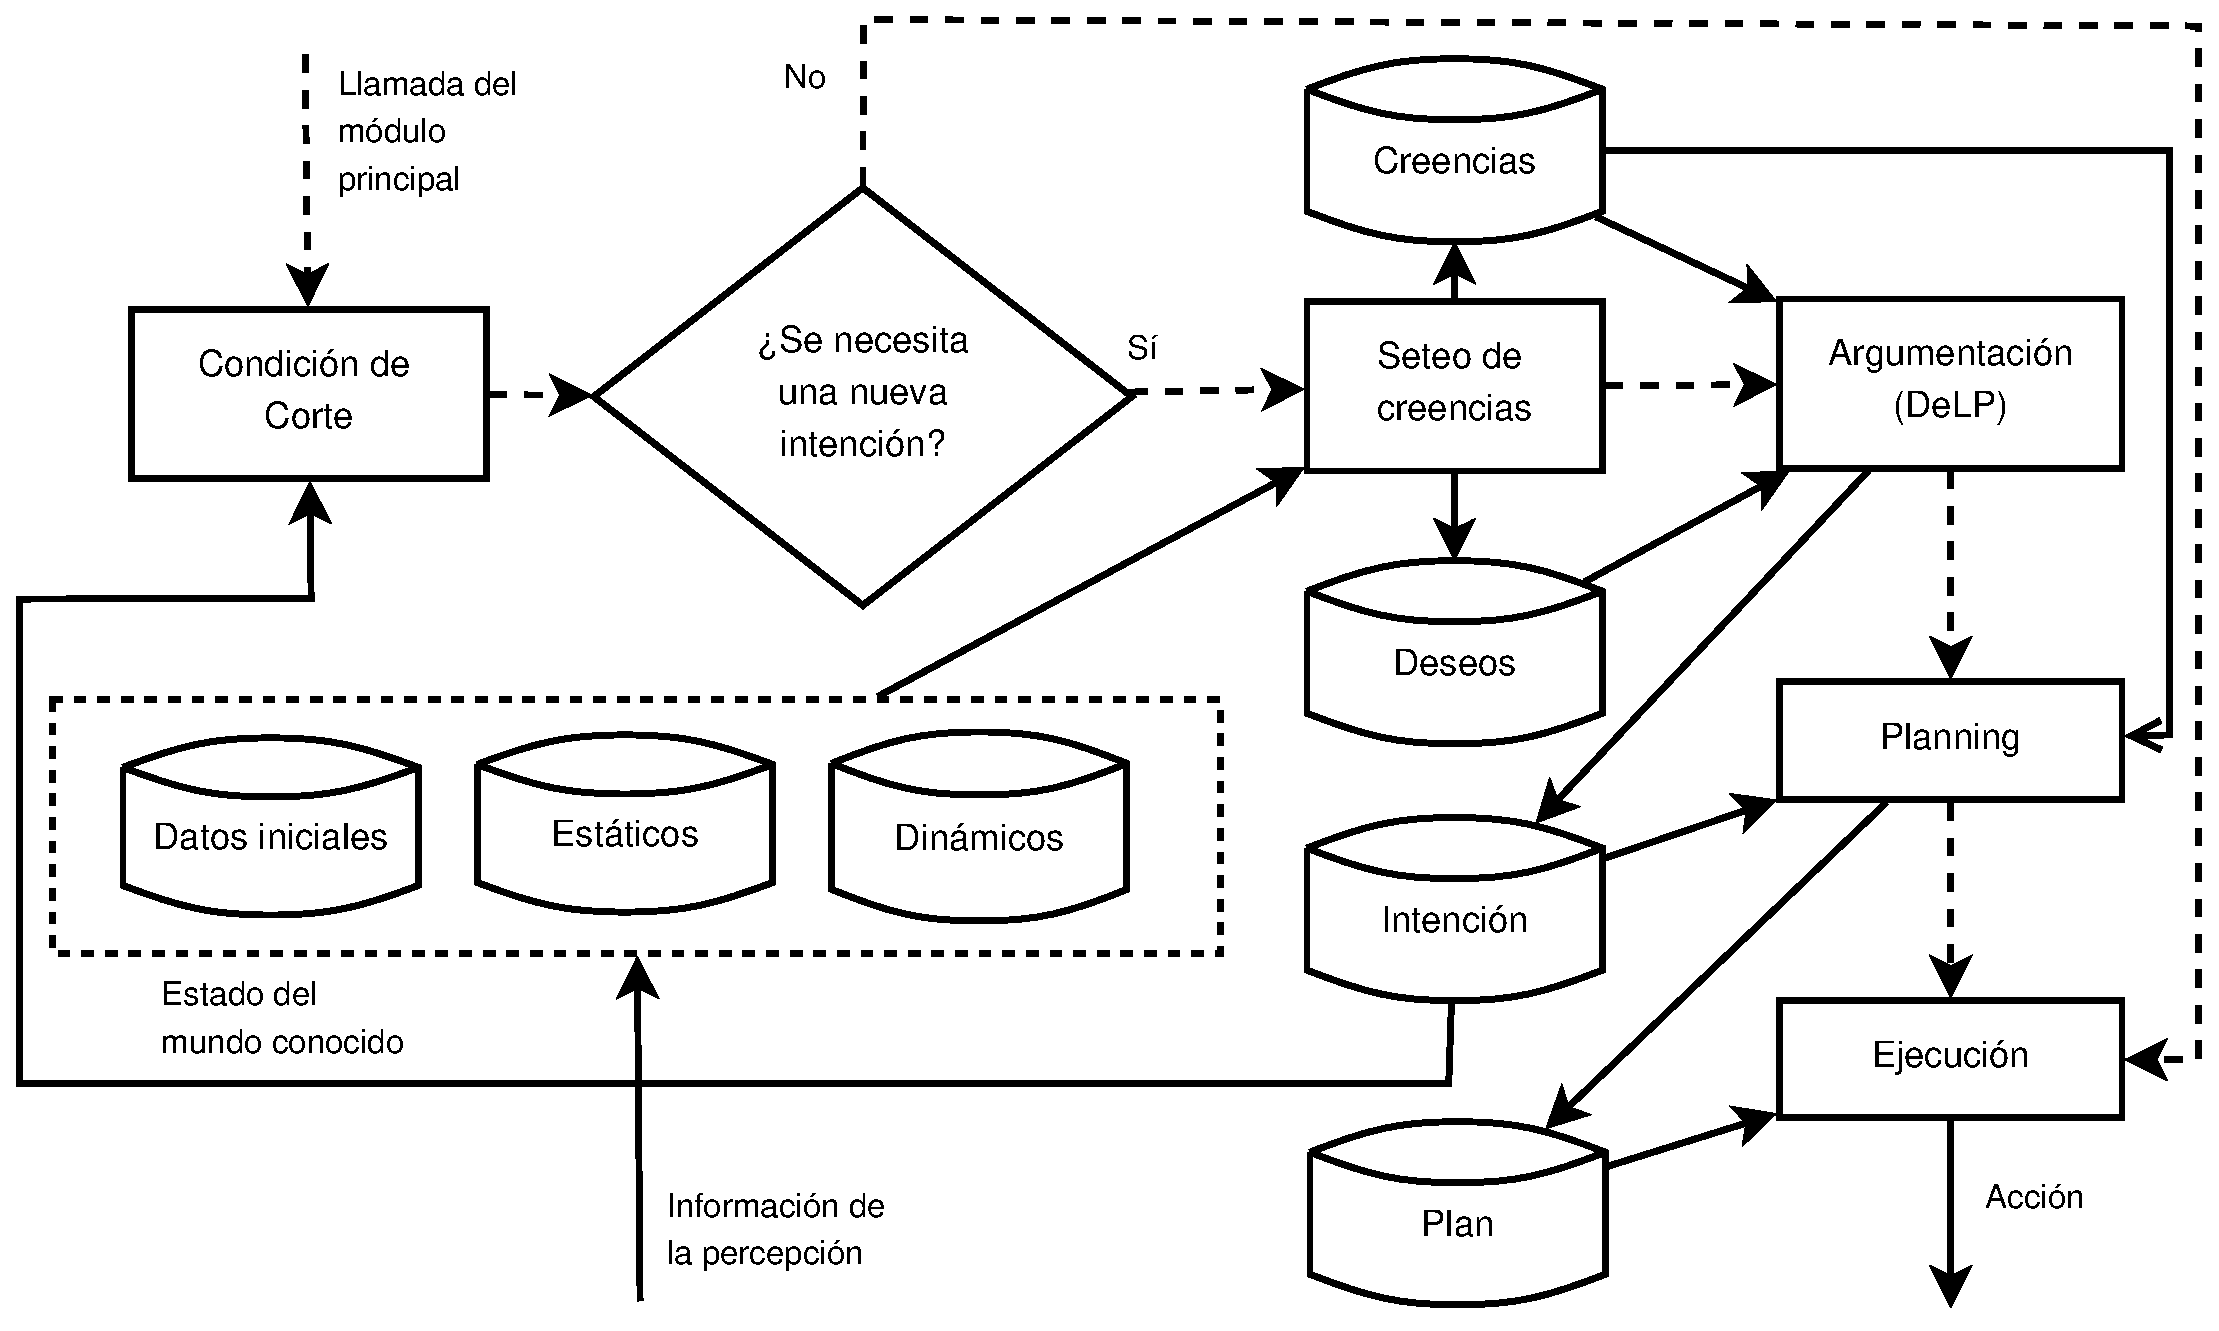
\includegraphics[scale=.3]{agent_prolog.eps}
 \caption{Diagrama de la arquitectura interna del agente, particularmente todo lo relacionado 
 con la toma de decisiones, hecha en Prolog. Las l�neas punteadas representan el 
 flujo de control, y las l�neas cont�nuas representan el flujo de datos.}
 \label{fig:agentProlog}
\end{figure}

\subsection{Seteo de creencias}

\label{sec:seteoCreencias}

El seteo de creencias es llevado a cabo cada vez que el agente se dispone a 
seleccionar una nueva intenci�n. Incluye la generaci�n de aquellos datos que pueden 
permitir al agente realizar una elecci�n lo m�s acertada posible. Se trata de 
inferencias realizadas en base al estado del escenario, es decir, aquella informaci�n 
que, como fue mencionado, es almacenada en \texttt{b/1}. No forma parte de este proceso 
la informaci�n proveniente de la percepci�n, ya que el estado del entorno es actualizado 
en cada turno de manera previa. Como se detalla a continuaci�n, distintos tipos de 
creencias pueden pueden estar relacionadas a distintos factores, como el rol del agente, 
su estado, o los deseos en an�lisis.

\subsubsection{Creencias generales}

Existe un conjunto de creencias que resultan de utilidad general para todo el proceso 
de decisi�n. Por esta raz�n, son las primeras en ser calculadas y almacenadas durante 
el seteo de creencias. Entre los datos incluidos, se encuentra el puntaje que est�n 
aportando las zonas armadas, la diferencia de puntos que puede producirse si el agente 
abandona su posici�n, y la seguridad que brindan las distintas ubicaciones posibles en 
cuanto a la presencia de agentes saboteadores enemigos. 

\subsubsection{Deseos}

Como se detallar� en el cap�tulo siguiente, el proceso de toma de decisi�n conlleva el 
pesaje de todos los posibles deseos del agente, y la posterior selecci�n del m�s beneficioso. 
Dichos deseos surgen de un conjunto predefinido, y pueden, seg�n sea el caso, estar 
instanciados con diferentes entidades del juego, como agentes o nodos. Para que esta 
selecci�n sea posible, es necesario determinar, de manera previa, qu� deseos e instanciaciones 
son realmente factibles, y por lo tanto deben ser tenidos en cuenta, y cuales pueden ser 
descartados anticipadamente.
Para esto se analizan distintas condiciones como, por ejemplo, la distancia a un nodo 
que no ha sido explorado. Si el nodo se encuentra a una distancia que supera una cota 
pre-establecida, entonces el deseo de explorar ese nodo no es contemplado.
Los deseos e instanciaciones considerados factibles son seteados en la base de conocimiento.

\begin{verbatim}
    b(posibleExplorar(vertex4)).
\end{verbatim}

\subsubsection{Creencias espec�ficas} % Seteo de beliefs para cada deseo.

Junto con los deseos a ser evaluados, es necesario incluir en la base de conocimiento 
un conjunto de creencias relacionadas a estos deseos. Entre las m�s importantes, se 
encuentran las distancias que existen desde la posici�n actual del agente a los distintos 
nodos de inter�s, y la diferencia de puntaje que se produce en caso que el agente se desplace 
a dichas ubicaciones. Estos datos resultan fundamentales, ya que afectan directamente la 
valuaci�n que se realiza de cada deseo, y por lo tanto la posterior selecci�n.

En esta etapa, tambi�n se produce el seteo de datos requeridos posteriormente, como son 
los caminos a los diferentes nodos analizados. Los algoritmos empleados para la b�squeda 
de caminos almacenan todos los caminos hallados, en forma de secuencia de acciones, de 
manera que la etapa de planificaci�n, ejecutada cuando se ha decidido una intenci�n, 
pueda ser realizada en forma simple e directa.

\subsubsection{Creencias especiales} % Seteo de beliefs en caso de agente deshabilitado.

Cuando el agente se encuentra en una situaci�n de peligro, esto es, no posee el rol de 
saboteador y hay un saboteador enemigo en su posici�n, o fue atacado en el turno anterior, 
el conjunto de creencias seteadas se reduce. En estos casos, s�lo son tenidos en cuenta 
los nodos vecinos, dado que representan las v�as de escape m�s r�pidas; son calculadas 
las distancias a estos (en cantidad de turnos), y las diferencias de puntaje que producir�a 
el desplazamiento del agente. Esto tiene el objetivo de minimizar la cantidad de deseos 
considerados: s�lo son evaluadas la posibilidad de permanecer en la misma ubicaci�n 
(si el beneficio en puntaje es considerable), y las distintas alternativas de defensa 
propia que pueden llevar al agente a superar el peligro.

\subsection{Argumentaci�n}

\label{sec:argumentacion}

Una vez finalizado el seteo de creencias, el agente procede a la selecci�n de la pr�xima 
intenci�n. Para esto, se toma cada uno de los deseos marcados como factibles en la base 
de conocimiento, y se los evalua junto a una serie de ``condiciones'' particulares. Se 
considera que existen razones para creer realizables s�lo aquellos deseos que satisfacen 
sus condiciones. Para estos, se obtiene un valor que representa su peso, en t�rminos del 
beneficio que conllevan para el equipo. El deseo que presenta el mayor peso entre los 
analizados, se convierte en la nueva meta del agente, la cual es almacenada hasta ser 
alcanzada o reemplazada.

Tanto la evaluaci�n como el pesaje de los deseos, son llevados a cabo empleando \textit{argumentaci�n} 
en un m�dulo especial, implementado con la ayuda de \textit{DeLP}. 
Detalles sobre la implementaci�n y como la argumentaci�n es aplicada en el proceso de 
razonamiento, son estudiados en el cap�tulo dedicado a la Toma de Decisiones. %referencia, cambiar nombre?

\subsection{Planificaci�n}

%\label{sec:planificacion}

La planificaci�n consiste en obtener la secuencia de acciones que llevan al cumplimiento 
de la intenci�n propuesta. Esta lista est� compuesta por las acciones que le permiten al 
agente posicionarse en el nodo deseado, y, en algunos casos, una acci�n concreta a realizar. 
Como se dijo anteriormente, en la etapa de seteo de creencias, todos los caminos hallados 
por el algoritmo de b�squeda son almacenados. Dicho algoritmo fue implementado de manera 
tal que los caminos no est�n constituidos por nodos o v�rtices, sino por una secuencia 
optimal de acciones, que tiene en cuenta no s�lo el nodo destino, sino tambi�n los recursos 
del agente, y la meta final a realizar (en caso de haber una acci�n final). De esta forma, 
cualquiera haya sido la intenci�n elegida, el agente cuenta en su base de conocimiento 
con el plan necesario para cumplirla. La planificaci�n se resume entonces a tomar las 
acciones correspondientes, y establecerlas efectivamente como el plan a seguir.

Alternativamente, esta etapa puede introducir ciertas acciones con el objetivo de optimizar 
el uso del turno. En aquellas situaciones en que el agente se dispone a permanecer inactivo, 
la acci�n nula (\texttt{skip}) puede ser reemplazada por la acci�n de recargar energ�a, si es que 
esta resulta m�s productiva.

\subsection{Ejecuci�n}

\label{sec:ejecucion}

Dado que el plan se encuentra almacenado de manera completa y ordenada, la ejecuci�n se 
realiza en forma directa. Se toma la pr�xima acci�n, es decir, la primera acci�n del plan 
restante, y se la retorna al m�dulo principal del programa. Este se encarga posteriormente 
de enviarla al entorno, para que se convierta finalmente en la siguiente acci�n realizada 
por el agente.

\subsection{Condici�n de corte}

\label{sec:condicionDeCorte}

Existen situaciones en las que el paso de los turnos genera que el cumplimiento de una 
meta se vuelva inalcanzable, innecesario, riesgoso, o menos productivo de lo previsto, por 
lo que resulta m�s beneficioso abortar el plan existente, y seleccionar una nueva intenci�n. 
�sta es una etapa de verificaci�n, que tiene como objetivo la detecci�n de este tipo de 
situaciones. Es ejecutada s�lo en aquellos turnos en los que el agente se encuentra 
siguiendo el plan de una intenci�n previamente determinada.

Cada deseo o esquema de deseo cuenta con una serie de \textbf{condiciones de corte}, que 
son evaluadas al inicio de cada turno, en caso de existir un plan establecido. Si se verifica 
que alguna de estas condiciones se satisface, entonces la intenci�n es descartada, y el 
agente ingresa en un nuevo proceso de selecci�n. 
Entre las condiciones de corte tenidas en cuenta, se encuentran: 

\begin{itemize}
	\item Que haya pasado una determinada cantidad de turnos desde el inicio del plan.
	\item Que el agente se encuentre deshabilitado.
	\item Que haya sido atacado o se encuentre amenazado por un enemigo.
	\item Que la meta haya sido alcanzada por un compa�ero de equipo.
\end{itemize}

\subsection{Re-planificaci�n}

%\label{sec:replanificaci�n}

La fase de re-planificaci�n consiste en elaborar nuevamente el plan que permite alcanzar 
la meta propuesta, sin modificar dicha meta. Este paso, como el anterior, se realiza en 
los turnos en los que el agente posee un plan pre-calculado. Dado que en estos turnos no 
es necesaria la obtenci�n de una nueva intenci�n, proceso que implica el mayor insumo de 
tiempo, la inclusi�n de la re-planificaci�n no afecta el funcionamiento normal del agente, 
en t�rminos de tiempo de ejecuci�n. 

Por el contrario, existe una mejora en el desempe�o del equipo, surgida de un mejor 
aprovechamiento de la informaci�n percibida. Los agentes actualizan su informaci�n sobre 
el estado del mundo en cada turno. Datos como el estado en que se hallan los recursos del 
agente, la incorporaci�n de nodos y arcos hasta el momento desconocidos, o las nuevas 
ubicaciones de los otros agentes, permiten elaborar planes m�s precisos y ajustados a la 
realidad que los originalmente dise�ados. As�, los agentes son capaces de cumplir sus 
metas con mayor facilidad, o abortarlas si es necesario.

\subsection{Coordinaci�n}

En esta tesis proponemos agregar una �ltima fase a la arquitectura de los agentes; el prop�sito de �sta es introducir, primero, una nueva etapa de comunicaci�n en la que cada uno de los agentes informa al resto de los miembros del equipo la decisi�n que ha tomado (es decir, cu�l es su intenci�n actual, y la acci�n inminente a realizar para intentar efectivizarla); y segundo, una etapa en la que se re-evaluar� la acci�n a realizar dependiendo tanto de cu�les sean las intenciones y acciones de los compa�eros de equipo, como de la fase actual del juego y las prioridades que los agentes tengan de acuerdo a ella.

\begin{figure}[h]
 \centering
 \includegraphics[scale=.3]{agent_architecture_expanded.eps}
 \caption{Diagrama de la arquitectura expandida. Se agrega una etapa en la que los agentes comunican la decisi�n tomada al resto de sus compa�eros (utilizando, por ejemplo, un proceso similar al servidor de percepciones). Las l�neas punteadas representan el flujo de control, y las l�neas cont�nuas representan el flujo de datos.}
 \label{fig:agentProlog}
\end{figure}

\begin{figure}[h]
 \centering
 \includegraphics[scale=.3]{agent_prolog_expanded.eps}
 \caption{Diagrama de la arquitectura interna expandida. Se propone agregar una fase de coordinaci�n, en la que, a partir de las decisiones tomadas por el resto de los compa�eros, el agente re-eval�a su propia acci�n a realizar.}
 \label{fig:agentProlog}
\end{figure}

En el cap�tulo siguiente detallaremos la propuesta de re-evaluaci�n de las decisiones tomadas por el agente. Es importante mencionar que esta fase agregada de coordinaci�n es, al menos en las versiones preeliminares desarrolladas, exigente en cuanto al tiempo de c�mputo; debido a las limitaciones temporales impuestas para los turnos de juego durante la competencia MAPC 2011, este agregado fue dise�ado y se comenz� su implementaci�n, pero al no conseguir la optimizaci�n suficiente como para que los agentes respondieran en el tiempo necesario, su utilizaci�n fue dejada de lado.
\chapter{Sistema de resoluci�n de conflictos}
En este cap�tulo se propondr� el marco te�rico y el esquema aplicativo del sistema de resoluci�n de conflictos a utilizar en el marco de MAPC. Es importante destacar que, si bien por limitaciones temporales nuestro equipo �nicamente implement� coordinaciones impl�citas entre las acciones de los agentes durante la competencia del a�o 2011, la idea de implementaci�n de un sistema de coordinaci�n m�s complejo y robusto fue parte de los planes desde el comienzo del trabajo.

\section{Informaci�n necesaria}
Despu�s de estudiar el flujo de informaci�n y el contenido de la base de conocimiento de cada uno de nuestros agentes, sabemos que en cada turno un agente conoce su conjunto completo de creencias, deseos, y tiene al menos una intenci�n persistente y bien determinada, al igual que \textit{al menos} una acci�n a realizar a futuro. Recordemos, adem�s, que gracias al Servidor de Percepciones cada agente tiene una visi�n unificada del mundo y conoce los roles, posiciones y caracter�sticas f�sicas de sus compa�eros de equipo.

Consideremos el agregado a la arquitectura mostrado; luego de esta nueva fase de comunicaci�n, todos los agentes conocen la decisi�n tomada por sus compa�eros de equipo, incluyendo tanto la intenci�n m�s fuerte como la acci�n a realizar por cada uno de ellos.  Toda esta informaci�n, en conjunto, puede ser utilizada con el fin de re-analizar concretamente cu�n potencialmente beneficiosa, peligrosa o perjudicial es la acci�n a realizar por el agente, y reconsiderar al respecto.

\section{Propuesta de coordinaci�n}

Mostraremos ahora la primer posibilidad de coordinaci�n propuesta; este sistema fue propuesto para ser utilizado durante la competencia MAPC 2011, y si bien no pudo ser presentado por falta de tiempo, existen algunas versiones en estado \textit{beta} ya implementadas.

Dado que el sistema provee suficiente flexibilidad como para permitir definir
distintas estrategias de resoluci�n de acuerdo a la t�ctica utilizada en la fase
actual del juego, el primer paso es escribir diferentes �rdenes de prioridad acordes a dichas fases. Es decir, el sistema de resoluci�n propuesto permite
modificar el comportamiento de los agentes de manera din�mica seg�n el estado
del juego, en lugar de resolver los potenciales conflictos siempre del mismo
modo. Los �rdenes de prioridad escritos indicar�n la importancia de las posibles intenciones de los agentes en una fase determinada del juego.

Una vez que contamos con los �rdenes de prioridad, el agente utiliza todo el
conocimiento de las caracter�sticas f�sicas y las intenciones y acciones
inminentes de sus compa�eros, y re-eval�a la propia. Es importante mencionar
que, en este esquema de coordinaci�n, cuando un agente decide que realizar la
acci�n que hab�a elegido deja de ser conveniente, pasa a actuar de manera
\textit{segura}, en el sentido de que realiza acciones que garantizan (o al
menos, maximizan las chances de) que no haya conflictos con otros agentes o
riesgo de p�rdida de puntos. Se detallar�n las potenciales acciones a realizar en \textit{modo seguro} en la secci�n siguiente, y m�s adelante analizaremos alternativas de acci�n que puedan dar a�n m�s r�dito.

\subsection{Clasificaci�n de conflictos}
Existen diferentes tipos de conflicto que los agentes pueden encontrar al
momento de reconsiderar su decisi�n respecto a la manera de actuar.

Resulta natural pensar, por ejemplo, que si dos o m�s agentes van a realizar una acci�n persiguiendo
una intenci�n id�ntica (y que dicha acci�n/intenci�n deba ser
realizada una �nica vez), entonces es un malgasto de recursos (energ�a) que
todos ellos la realicen. Un ejemplo de este caso ocurre cuando dos agentes
cualesquiera tienen como intenci�n survey($X_{i}$), cuando dos exploradores
tienen como intenci�n probear($X_{i}$), o cuando dos inspectores tienen como
intenci�n inspect($X_{i}$), para el mismo \textit{i}. En cualquiera de estos
casos, resulta evidente que s�lo uno de los agentes deber�a llevar a cabo la
acci�n. El criterio espec�fico para decidir cu�l de ellos la realiza puede ser
definido de muchas maneras; el propuesto para la competencia fue dejar que el
agente que pudiera efectivizar la intenci�n en menor cantidad de turnos
realizara la acci�n, y en caso de empate, dejar que el que tuviera m�s energ�a
fuera el ganador. Si ambas condiciones resultaran en empate, el ganador se
determina por orden lexicogr�fico, pasando todos los perdedores a actuar en \textit{modo seguro}.

Sin embargo, no todos los casos en los que dos o m�s agentes tengan exactamente
la misma intenci�n resultan conflictivos: por ejemplo, dos saboteadores pueden
querer atacar de manera simult�nea a un mismo enemigo. Esta situaci�n da lugar a
la clasificaci�n de todas las intenciones en dos tipos: \textit{cooperativas} y
\textit{excluyentes}.

Por �ltimo, existen conflictos m�s complejos para su detecci�n y
resoluci�n; por ejemplo, que dos agentes decidan moverse para
expandir una zona ya dominada, y que el movimiento sincronizado resulte en la
p�rdida de la zona.

A continuaci�n, analizaremos c�mo se detectan y resuelven todos estos
conflictos.

\subsection{Detecci�n de conflictos}

Una vez finalizada la segunda fase de comunicaci�n, cada agente considera las
intenciones y acciones a realizar de los dem�s miembros del equipo en busca de
potenciales conflictos.

El primer paso consiste en ordenar a los agentes de acuerdo al orden de prioridad establecido a las intenciones para la fase del juego actual. La intenci�n que cada agente persigue ser� utilizada para definir, en caso de conflicto, cu�les de los agentes podr�n continuar y cu�les deber�n realizar otro tipo de acci�n que no resulte perjudicial.%bla bla bla bla bla

El paso siguiente es verificar si otros agentes tienen una
intenci�n \textit{excluyente} que coincida con la propia. Si ese es el caso, se
eval�a cu�l de dichos agentes se encuentra en mejor estado para efectivizar
la intenci�n (de acuerdo a, como se mencion� antes, la cantidad de turnos
que necesitar� para efectivizarla, seguido en caso de empate por la energ�a de cada uno de ellos, y por �ltimo seg�n el orden lexicogr�fico de sus nombres).
Por razones de optimizaci�n, en las versiones beta ya implementadas del sistema los agentes proveen en la �ltima fase de comunicaci�n la cantidad de turnos que suponen necesitar para efectivizar la intenci�n (considerando siempre el mejor caso; es decir, que no ocurran condiciones de corte, ataques enemigos, o cambios de plan repentinos).% mencionar que en versiones futuras se puede incluir TODO EL PLAN de los agentes (es decir, todos los pasos que van a seguir), para posiblemente argumentar sobre la mejor decisi�n con eso (?)

A continuaci�n, en caso de que la etapa anterior no haya detectado ning�n conflicto, se pasa a la fase m�s compleja de la detecci�n; dado que cada agente que provoque cambios en su posici�n en el mapa puede afectar el control de las zonas dominadas, el sistema realiza una simulaci�n progresiva de los puntos que el equipo puede obtener de acuerdo a las nuevas hipot�ticas posiciones de cada agente. Esta simulaci�n es llamada \textit{progresiva} porque se realiza corriendo una instancia del algoritmo de coloreo por cada nueva posici�n hipot�tica de los agentes. Recordando que los miembros del equipo se encuentran ordenados de acuerdo a la prioridad de sus intenciones, el sistema comienza calculando el puntaje seg�n las posiciones originales de todos los agentes \textit{excepto el que tiene la mayor prioridad para moverse}; a partir de este puntaje base, se vuelve a correr el algoritmo de coloreo con la nueva posici�n hipot�tica del segundo agente mejor priorizado; este puntaje se compara con el puntaje base del primer c�lculo,% mayor o igual? definir threshold?
y si es mayor o igual, pasa a ser el nuevo puntaje de referencia.

Los c�lculos contin�an repiti�ndose posicionando a cada agente en su nueva posici�n hipot�tica. Si efectivamente la acci�n mejora o mantiene igual el puntaje obtenido en el turno, entonces se considera que esta acci�n no resulta perjudicial para el equipo. En caso contrario, se interpreta que la acci�n a tomar por el agente conflictivo es peligrosa, y ese agente debe pasar a actuar en \textit{modo seguro}; por lo tanto, la siguiente instancia del algoritmo para calcular el puntaje del equipo se corre con el agente conflictivo en su posici�n original, y continuando con la nueva posici�n hipot�tica del siguiente agente, hasta haber evaluado las acciones de todos ellos.

\subsection{Resoluci�n de conflictos}

A continuaci�n detallaremos el m�todo utilizado para resolver los conflictos detectados por el sistema, as� como algunas alternativas de acci�n en trabajos a futuro.

\subsubsection{Acciones seguras}

En caso de que en la fase de resoluci�n de conflictos un agente detecte que su acci�n a realizar es perjudicial, el dise�o actual distribuido hace que el agente tenga la responsabilidad de actuar en \textit{modo seguro}. Este modo de actuar implica realizar acciones que puedan beneficiar de alguna manera al equipo, pero sin correr riesgo de p�rdida de puntaje global; es decir, el agente realiza cualquier acci�n \textit{que no implique movimiento} y suponga alg�n tipo de mejora a no realizar ninguna acci�n. Un ejemplo v�lido de acci�n segura para todos los roles de agente es la acci�n \textit{recharge}; por lo tanto, si el movimiento de un agente puede causar p�rdida mayor de puntos, �ste puede limitarse a recuperar su energ�a y buscar otra acci�n �til el turno siguiente. La acci�n \textit{survey} tambi�n resulta extremadamente �til en esta situaci�n, dado que proveer� informaci�n del mapa a todos los dem�s agentes en el turno siguiente gracias al Servidor de Percepciones. Por �ltimo, el impedimento para desplazarse convierte al turno en una excelente oportunidad para que los agentes realicen la acci�n \textit{buy} para mejorar sus caracter�sticas f�sicas, en caso de que el equipo tenga cr�ditos suficientes.

Considerando, adem�s, los roles de los agentes, podemos definir otras acciones \textit{seguras}: los exploradores pueden realizar la acci�n \textit{probe} sobre el nodo en el que se encuentran parados sin ning�n tipo de riesgo, aportando adem�s informaci�n valiosa sobre el mapa a sus compa�eros. Los saboteadores tienen la posibilidad de atacar enemigos cercanos sin moverse, convirti�ndola tambi�n en una acci�n \textit{segura}. Los inspectores pueden realizar la acci�n \textit{inspect} sobre cualquier enemigo cercano, los reparadores pueden ayudar a sus compa�eros a recuperar su salud sin desplazarse, y por �ltimo, los reparadores, saboteadores y sentinelas pueden realizar \textit{parry} para intentar prevenir ataques enemigos.

Si bien probablemente ninguna de las acciones alternativas resulte �ptima en vista del estado del escenario, se ha comprobado emp�ricamente luego de diez mil simulaciones de trescientos cincuenta turnos cada una, que el cambio a \textit{modo seguro} de los agentes resulta extremadamente beneficioso para el puntaje del equipo.% esto quiz�s se pueda poner en las conclusiones!

\subsubsection{Trabajo a futuro}

Como se mencion� anteriormente, el actual sistema de resoluci�n de conflictos mejora el comportamiento de los agentes y el puntaje obtenido por el equipo. Sin embargo, dado que las acciones tomadas por los agentes conflictivos generalmente no resultan �ptimas, es evidente que hay mucho trabajo por realizar a futuro en la etapa de reconsideraci�n de acciones.

La primer mejora posible respecto al sistema actual consiste en hacer que los agentes comuniquen no s�lo la cantidad de pasos de simulaci�n que esperan necesitar para efectivizar su intenci�n actual, sino tambi�n todo el plan que formularon para ello; de esta manera, los agentes pueden realizar predicciones m�s efectivas respecto al movimiento de sus compa�eros y la cantidad de puntos que puede obtener el equipo en corto y mediano plazo, considerando la eventual posibilidad de sacrificar puntos en turnos cercanos para conseguir un mayor puntaje global a mediano plazo.

Otra mejora que surge naturalmente en el sistema es no limitar a los agentes a realizar �nicamente acciones \textit{seguras}; como punto de partida, es posible hacer que los agentes agreguen a su base de conocimiento el argumento \textit{NO X}, siendo \textit{X} la acci�n conflictiva detectada por el sistema, y realizar el proceso argumentativo una vez m�s, y repetir la detecci�n de conflicto. En corto tiempo se llegar�a a un estado en el que todos los agentes realizan la que consideran la mejor acci�n sin perjudicar al resto de sus compa�eros mejor priorizados, y a partir de una decisi�n tomada con mayor criterio que el de selecci�n de una acci�n \textit{segura}. Al comienzo del turno siguiente, el argumento agregado podr�a ser eliminado, dejando la chance de que el agente reconsidere realizar la acci�n nuevamente con la eventual posibilidad de no perjudicar a sus compa�eros.

Por �ltimo, un cambio m�s radical pero muy interesante a nivel acad�mico consiste en modificar la cantidad de informaci�n compartida por los agentes a partir del Servidor de Percepciones, haciendo que los agentes no conozcan la informaci�n sobre las caracter�sticas f�sicas de sus compa�eros. Luego de la fase de toma de decisi�n por parte de los agentes, una vez que se detectan conflictos por intenciones \textit{excluyentes}, los agentes involucrados podr�an utilizar Argumentaci�n Rebatible para decidir cu�l es m�s apto para realizar la tarea; y mejor a�n, ser�a posible implementar negociaci�n entre los agentes para intentar obtener ayuda de los propios compa�eros. Por otro lado, tambi�n podr�a utilizarse Argumentaci�n Rebatible para resolver los conflictos m�s complejos utilizando como argumentos las predicciones de cada uno de los agentes del estado del escenario a futuro a partir de sus acciones.
\chapter{Conclusiones}

Podemos concluir que ...
\begin{thebibliography}{99}
\addcontentsline{toc}{chapter}{Bibliograf�a}
\bibitem{jade99}
  F. Bellifemine, A. Poggi, G. Rimassa,
  \emph{JADE - A FIPA-compliant agent framework}.
  CSELT internal technical report,
  1999.
\bibitem{dev01}
  F. Bellifemine, A. Poggi, G. Rimassa,
  \emph{Developing multi-agent systems with a FIPA-compliant agent framework}.
  Software - Practice And Experience,
  2001.
\bibitem{coord00}
  R. S. Cost, Y. Labrou, T. Finin,
  \emph{Coordinating Agents using Agent Communication Languages Conversations}.
  2000. 	
\bibitem{apl03}
  Dastani et al.,
  \emph{A Programming Language for Cognitive Agents: Goal Directed 3APL}.
  Proceedings of the First Workshop on Programming Multiagent Systems: Languages, frameworks, techniques, and tools,
  2003.
\bibitem{coop96}
  Doran et al.,
  \emph{On Cooperation in Multi-Agent Systems. The Knowledge Engineering Review}.
  1996.
\bibitem{delp04}
  A. J. Garc�a, G. R. Simari,
  \emph{Defeasible logic programming: An argumentative approach}.
  Journal of Theory and Practice of Logic Programming,
  2004.
\bibitem{int05}
  A. J. Garc�a, M. Tucat, G. R. Simari,
  \emph{Interaction Primitives for Implementing Multi-agent Systems}.
  Interaction Primitives for Implementing Multi-agent Systems,
  2005.
\bibitem{mult99}
  M. Huhns, L. Stephens,
  \emph{Multiagent Systems and Societies of Agents}.
  Multiagent Systems: A Modern Approach to Distributed Artificial Intelligence,
  1999.
\bibitem{arg98}
  N. R. Jennings et al.,
  \emph{Argumentation-Based Negotiation}.
  Proceedings of the International Workshop on Multi-Agent Systems,
  1998.
\bibitem{soc99}
  S. Kalenka, N. R. Jennings,
  \emph{Socially Responsible Decision Making by Autonomous Agents}.
  Proceedings of the 5th International Colloquium on Cognitive Science,
  1999.
\bibitem{neg96}
  J. M�ller,
  \emph{Negotiation Principles}.
  Foundations of Distributed Artificial Intelligence,
  1996.
\bibitem{mod91}
  A. Rao, M. Georgeff,
  \emph{Modeling rational agents within a BDI-architecture}.
  Proceedings of the Second International Conference on Principles of Knowledge Representation and Reasoning,
  1991.
\bibitem{bdi95}
  A. S. Rao, M. P. Georgeff,
  \emph{BDI Agents: From Theory to Practice}.
  Proceedings of the First International Conference on Multi-Agent Systems,
  1995.
\bibitem{arg02}
  S. V. Rueda, A. J. Garc�a, G. R. Simari,
  \emph{Argument-based Negotiation among BDI Agents}.
  Journal of Computer Science and Technology,
  2002.
\bibitem{ia99}
  M. Wooldridge,
  \emph{Intelligent Agents}.
  Multiagent Systems, The MIT Press,
  1999.
\bibitem{brat99}
    M. E. Bratman,
    \emph{Intention, Plans, and Practical Reason}.
    Cambridge University Press,
    1999.
\bibitem{searle1985}
	J.R. Searle,
  \emph{Intentionality, an Essay in the Philosophy of Mind}.
  Cambridge University Press,
  1983.

\end{thebibliography}

\end{document}
